% $HeadURL: https://sbgn.svn.sourceforge.net/svnroot/sbgn/ProcessDiagram/tags/L1V1.3Full/sources/stateVariable.tex $

\subsection{Glyph: \glyph{State variable}}
\label{sec:stateVariable}

Many biological entities, such as molecules, can exist in different \emph{states}, meaning different physical or informational configurations.  These states can arise for a variety of reasons.  For example, macromolecules can be subject to post-synthesis modifications, wherein residues of the macromolecules (amino acids, nucleosides, or glucid residues) are modified through covalent linkage to other chemicals.  Other examples of states are alternative conformations as in the closed/open/desensitized conformations of a transmembrane channel, and the active/inactive forms of an enzyme.

SBGN provides a means of associating one or more \glyph{state variables} with an entity; each such variable can be used to represent a dimension along which the state of the overall entity can vary.  When an entity can exist in different states, the state of the whole entity (\ie the SBGN object) can be described by the current values of all its \glyph{state variables}, and the values of the \glyph{state variables} of all its possible components, recursively. A \glyph{state variable} is represented by an elliptical container overlapping the border of the \glyph{EPN} being annotated.

\begin{figure}[H]
  \centering
  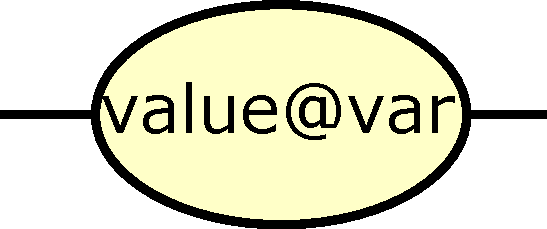
\includegraphics[scale = 0.3, trim = 0 0 0 0.25in]{images/stateVariable}
  \caption{The \PD glyph for \glyph{state variable}.}
  \label{fig:state-var}
\end{figure}
 
A \glyph{state variable} does not necessarily have to be Boolean-valued.  For example, an ion channel can possess several conductance states; a receptor can be inactive, active and desensitized; and so on.  As another example, a \glyph{state variable} ``ubiquitin'' could also carry numerical values corresponding to the number of ubiquitin molecules present in the tail.  However, in all cases, a \glyph{state variable} on an EPN can only take \emph{one} defined value.  Further, an EPN's \glyph{state variable} should always be displayed and always set to a value.  An ``empty'' \glyph{state variable} is a \glyph{state variable} that is set to the value ``unset'', it is not a \glyph{state variable} with no value. Note that the value ``unset'' is \emph{not} synonymous to ``any value'' or ``unknown value''.


